\documentclass[]{krantz}
\usepackage{lmodern}
\usepackage{amssymb,amsmath}
\usepackage{ifxetex,ifluatex}
\usepackage{fixltx2e} % provides \textsubscript
\ifnum 0\ifxetex 1\fi\ifluatex 1\fi=0 % if pdftex
  \usepackage[T1]{fontenc}
  \usepackage[utf8]{inputenc}
\else % if luatex or xelatex
  \ifxetex
    \usepackage{mathspec}
  \else
    \usepackage{fontspec}
  \fi
  \defaultfontfeatures{Ligatures=TeX,Scale=MatchLowercase}
\fi
% use upquote if available, for straight quotes in verbatim environments
\IfFileExists{upquote.sty}{\usepackage{upquote}}{}
% use microtype if available
\IfFileExists{microtype.sty}{%
\usepackage[]{microtype}
\UseMicrotypeSet[protrusion]{basicmath} % disable protrusion for tt fonts
}{}
\PassOptionsToPackage{hyphens}{url} % url is loaded by hyperref
\usepackage[unicode=true]{hyperref}
\PassOptionsToPackage{usenames,dvipsnames}{color} % color is loaded by hyperref
\hypersetup{
            pdftitle={Limitations of Interpretable Machine Learning Methods},
            colorlinks=true,
            linkcolor=Maroon,
            citecolor=Blue,
            urlcolor=Blue,
            breaklinks=true}
\urlstyle{same}  % don't use monospace font for urls
\usepackage{natbib}
\bibliographystyle{apalike}
\usepackage{color}
\usepackage{fancyvrb}
\newcommand{\VerbBar}{|}
\newcommand{\VERB}{\Verb[commandchars=\\\{\}]}
\DefineVerbatimEnvironment{Highlighting}{Verbatim}{commandchars=\\\{\}}
% Add ',fontsize=\small' for more characters per line
\usepackage{framed}
\definecolor{shadecolor}{RGB}{248,248,248}
\newenvironment{Shaded}{\begin{snugshade}}{\end{snugshade}}
\newcommand{\KeywordTok}[1]{\textcolor[rgb]{0.13,0.29,0.53}{\textbf{#1}}}
\newcommand{\DataTypeTok}[1]{\textcolor[rgb]{0.13,0.29,0.53}{#1}}
\newcommand{\DecValTok}[1]{\textcolor[rgb]{0.00,0.00,0.81}{#1}}
\newcommand{\BaseNTok}[1]{\textcolor[rgb]{0.00,0.00,0.81}{#1}}
\newcommand{\FloatTok}[1]{\textcolor[rgb]{0.00,0.00,0.81}{#1}}
\newcommand{\ConstantTok}[1]{\textcolor[rgb]{0.00,0.00,0.00}{#1}}
\newcommand{\CharTok}[1]{\textcolor[rgb]{0.31,0.60,0.02}{#1}}
\newcommand{\SpecialCharTok}[1]{\textcolor[rgb]{0.00,0.00,0.00}{#1}}
\newcommand{\StringTok}[1]{\textcolor[rgb]{0.31,0.60,0.02}{#1}}
\newcommand{\VerbatimStringTok}[1]{\textcolor[rgb]{0.31,0.60,0.02}{#1}}
\newcommand{\SpecialStringTok}[1]{\textcolor[rgb]{0.31,0.60,0.02}{#1}}
\newcommand{\ImportTok}[1]{#1}
\newcommand{\CommentTok}[1]{\textcolor[rgb]{0.56,0.35,0.01}{\textit{#1}}}
\newcommand{\DocumentationTok}[1]{\textcolor[rgb]{0.56,0.35,0.01}{\textbf{\textit{#1}}}}
\newcommand{\AnnotationTok}[1]{\textcolor[rgb]{0.56,0.35,0.01}{\textbf{\textit{#1}}}}
\newcommand{\CommentVarTok}[1]{\textcolor[rgb]{0.56,0.35,0.01}{\textbf{\textit{#1}}}}
\newcommand{\OtherTok}[1]{\textcolor[rgb]{0.56,0.35,0.01}{#1}}
\newcommand{\FunctionTok}[1]{\textcolor[rgb]{0.00,0.00,0.00}{#1}}
\newcommand{\VariableTok}[1]{\textcolor[rgb]{0.00,0.00,0.00}{#1}}
\newcommand{\ControlFlowTok}[1]{\textcolor[rgb]{0.13,0.29,0.53}{\textbf{#1}}}
\newcommand{\OperatorTok}[1]{\textcolor[rgb]{0.81,0.36,0.00}{\textbf{#1}}}
\newcommand{\BuiltInTok}[1]{#1}
\newcommand{\ExtensionTok}[1]{#1}
\newcommand{\PreprocessorTok}[1]{\textcolor[rgb]{0.56,0.35,0.01}{\textit{#1}}}
\newcommand{\AttributeTok}[1]{\textcolor[rgb]{0.77,0.63,0.00}{#1}}
\newcommand{\RegionMarkerTok}[1]{#1}
\newcommand{\InformationTok}[1]{\textcolor[rgb]{0.56,0.35,0.01}{\textbf{\textit{#1}}}}
\newcommand{\WarningTok}[1]{\textcolor[rgb]{0.56,0.35,0.01}{\textbf{\textit{#1}}}}
\newcommand{\AlertTok}[1]{\textcolor[rgb]{0.94,0.16,0.16}{#1}}
\newcommand{\ErrorTok}[1]{\textcolor[rgb]{0.64,0.00,0.00}{\textbf{#1}}}
\newcommand{\NormalTok}[1]{#1}
\usepackage{longtable,booktabs}
% Fix footnotes in tables (requires footnote package)
\IfFileExists{footnote.sty}{\usepackage{footnote}\makesavenoteenv{long table}}{}
\usepackage{graphicx,grffile}
\makeatletter
\def\maxwidth{\ifdim\Gin@nat@width>\linewidth\linewidth\else\Gin@nat@width\fi}
\def\maxheight{\ifdim\Gin@nat@height>\textheight\textheight\else\Gin@nat@height\fi}
\makeatother
% Scale images if necessary, so that they will not overflow the page
% margins by default, and it is still possible to overwrite the defaults
% using explicit options in \includegraphics[width, height, ...]{}
\setkeys{Gin}{width=\maxwidth,height=\maxheight,keepaspectratio}
\IfFileExists{parskip.sty}{%
\usepackage{parskip}
}{% else
\setlength{\parindent}{0pt}
\setlength{\parskip}{6pt plus 2pt minus 1pt}
}
\setlength{\emergencystretch}{3em}  % prevent overfull lines
\providecommand{\tightlist}{%
  \setlength{\itemsep}{0pt}\setlength{\parskip}{0pt}}
\setcounter{secnumdepth}{5}
% Redefines (sub)paragraphs to behave more like sections
\ifx\paragraph\undefined\else
\let\oldparagraph\paragraph
\renewcommand{\paragraph}[1]{\oldparagraph{#1}\mbox{}}
\fi
\ifx\subparagraph\undefined\else
\let\oldsubparagraph\subparagraph
\renewcommand{\subparagraph}[1]{\oldsubparagraph{#1}\mbox{}}
\fi

% set default figure placement to htbp
\makeatletter
\def\fps@figure{htbp}
\makeatother

\usepackage{booktabs}
\usepackage{longtable}
\usepackage[bf,singlelinecheck=off]{caption}

\usepackage{framed,color}
\definecolor{shadecolor}{RGB}{248,248,248}

\renewcommand{\textfraction}{0.05}
\renewcommand{\topfraction}{0.8}
\renewcommand{\bottomfraction}{0.8}
\renewcommand{\floatpagefraction}{0.75}

\renewenvironment{quote}{\begin{VF}}{\end{VF}}
\let\oldhref\href
\renewcommand{\href}[2]{#2\footnote{\url{#1}}}

\makeatletter
\newenvironment{kframe}{%
\medskip{}
\setlength{\fboxsep}{.8em}
 \def\at@end@of@kframe{}%
 \ifinner\ifhmode%
  \def\at@end@of@kframe{\end{minipage}}%
  \begin{minipage}{\columnwidth}%
 \fi\fi%
 \def\FrameCommand##1{\hskip\@totalleftmargin \hskip-\fboxsep
 \colorbox{shadecolor}{##1}\hskip-\fboxsep
     % There is no \\@totalrightmargin, so:
     \hskip-\linewidth \hskip-\@totalleftmargin \hskip\columnwidth}%
 \MakeFramed {\advance\hsize-\width
   \@totalleftmargin\z@ \linewidth\hsize
   \@setminipage}}%
 {\par\unskip\endMakeFramed%
 \at@end@of@kframe}
\makeatother

\renewenvironment{Shaded}{\begin{kframe}}{\end{kframe}}

\usepackage{makeidx}
\makeindex

\urlstyle{tt}

\usepackage{amsthm}
\makeatletter
\def\thm@space@setup{%
  \thm@preskip=8pt plus 2pt minus 4pt
  \thm@postskip=\thm@preskip
}
\makeatother

\frontmatter

\title{Limitations of Interpretable Machine Learning Methods}
\date{2019-05-20}

\begin{document}
\maketitle

% you may need to leave a few empty pages before the dedication page

%\cleardoublepage\newpage\thispagestyle{empty}\null
%\cleardoublepage\newpage\thispagestyle{empty}\null
%\cleardoublepage\newpage
\thispagestyle{empty}

\begin{center}
\end{center}

\setlength{\abovedisplayskip}{-5pt}
\setlength{\abovedisplayshortskip}{-5pt}

{
\hypersetup{linkcolor=black}
\setcounter{tocdepth}{2}
\tableofcontents
}
\listoftables
\listoffigures
\chapter*{Preface}\label{preface}


This project explains the limitations of current approaches in
interpretable machine learning, such as partial dependence plots (PDP,
Accumulated Local Effects (ALE), permutation feature importance,
leave-one-covariate out (LOCO) and local interpretable model-agnostic
explanations (LIME). All of those methods can be used to explain the
behavior and predictions of trained machine learning models. The
interpretation methods might not work well in the following cases:

\begin{itemize}
\tightlist
\item
  if a model models interactions (e.g.~when a random forest is used)
\item
  if features strongly correlate with each other
\item
  if the model does not correctly model causal relationships
\item
  if parameters of the interpretation method are not set correctly
\end{itemize}

\section*{Structure of the book}\label{structure-of-the-book}


TODO

\mainmatter

\chapter{Introduction}\label{introduction}

Here is some text

\section{This is a smaller title}\label{this-is-a-smaller-title}

We have a nice figure in Figure \ref{fig:hello}, and also a table in
Table \ref{tab:iris}.

\begin{Shaded}
\begin{Highlighting}[]
\KeywordTok{par}\NormalTok{(}\DataTypeTok{mar =} \KeywordTok{c}\NormalTok{(}\DecValTok{4}\NormalTok{, }\DecValTok{4}\NormalTok{, }\DecValTok{1}\NormalTok{, .}\DecValTok{1}\NormalTok{))}
\KeywordTok{plot}\NormalTok{(cars, }\DataTypeTok{pch =} \DecValTok{19}\NormalTok{)}
\end{Highlighting}
\end{Shaded}

\begin{figure}
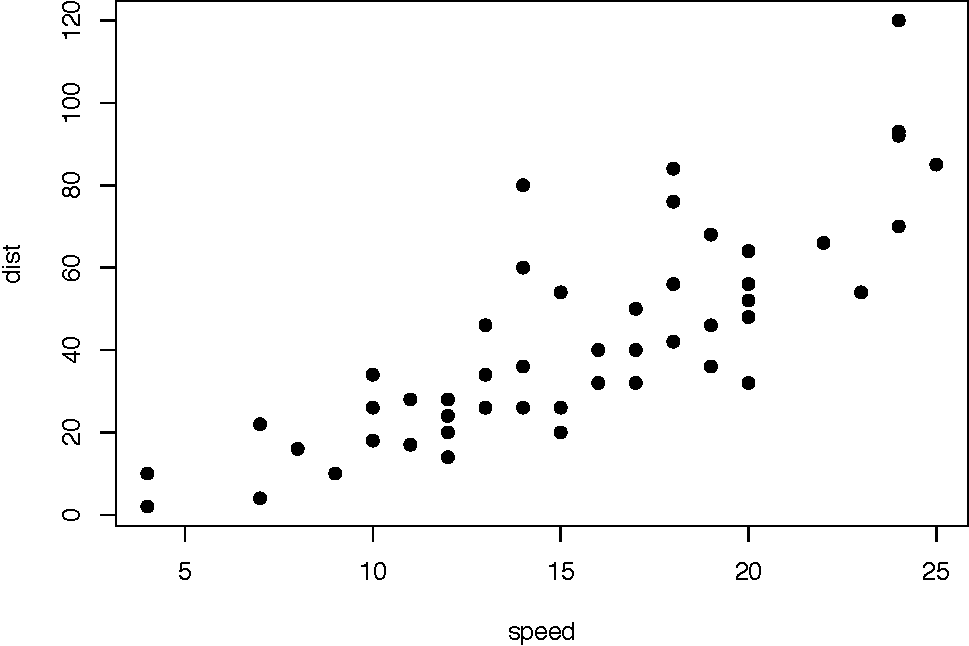
\includegraphics[width=0.9\linewidth]{book_files/figure-latex/hello-1} \caption{Hello World!}\label{fig:hello}
\end{figure}

\begin{Shaded}
\begin{Highlighting}[]
\NormalTok{knitr}\OperatorTok{::}\KeywordTok{kable}\NormalTok{(}
  \KeywordTok{head}\NormalTok{(iris), }\DataTypeTok{caption =} \StringTok{'The boring iris data.'}\NormalTok{,}
  \DataTypeTok{booktabs =} \OtherTok{TRUE}
\NormalTok{)}
\end{Highlighting}
\end{Shaded}

\begin{table}[t]

\caption{\label{tab:iris}The boring iris data.}
\centering
\begin{tabular}{rrrrl}
\toprule
Sepal.Length & Sepal.Width & Petal.Length & Petal.Width & Species\\
\midrule
5.1 & 3.5 & 1.4 & 0.2 & setosa\\
4.9 & 3.0 & 1.4 & 0.2 & setosa\\
4.7 & 3.2 & 1.3 & 0.2 & setosa\\
4.6 & 3.1 & 1.5 & 0.2 & setosa\\
5.0 & 3.6 & 1.4 & 0.2 & setosa\\
\addlinespace
5.4 & 3.9 & 1.7 & 0.4 & setosa\\
\bottomrule
\end{tabular}
\end{table}

\chapter{Partial Dependence Plots (PDP) and Individual Conditional
Expectation (ICE)
Curves}\label{partial-dependence-plots-pdp-and-individual-conditional-expectation-ice-curves}

\section{Partial Dependence Plots
(PDP)}\label{partial-dependence-plots-pdp}

The Partial Dependence Plot (PDP) is a rather intuitive and
easy-to-understand visualization of the features' impact on the
predicted outcome. It maps the marginal effect of the selected
variable(s) and can reveal the nature of dependence structure between
target and individual feature variable\footnote{Molnar. ``Interpretable
  Machine Learning''.
  \url{https://christophm.github.io/interpretable-ml-book/simple.html}.}.

The underlying function can be described as follows:

Let \(x_S\) be the set of features of interest for the PDP and \(x_C\)
the complement set which contains all other features. While the general
model function \(f(x) = f(x_S, x_C)\) depends on all input variables,
the partial dependence function marginalizes over the feature
distribution in set C:\footnote{Hastie, Tibshirani, Friedman. The
  Elements of Statistical Learning. Springer.
  \url{https://web.stanford.edu/~hastie/ElemStatLearn/printings/ESLII_print12.pdf}.}

\[f_{x_S}(x_S) = \mathbb{E}_{x_C}[f(x_S, x_C)]\]

The partial dependence function can be estimated by averaging the actual
feature values of \(x_C\) in the training data at given values of
\(x_S\) or, in other words, it computes the marginal effect of \(x_S\)
on the prediction. In order to derive realistic results, a major
assumption of the PDP is that the features in \(x_S\) and \(x_C\) are
independent and thus uncorrelated.\footnote{Hastie, Tibshirani,
  Friedman. The Elements of Statistical Learning. Springer.
  \url{https://web.stanford.edu/~hastie/ElemStatLearn/printings/ESLII_print12.pdf}.}

\[\hat{f}_{x_S}(x_S)=\frac{1}{n}\sum_{i=1}^{n}f(x_S, x^{(i)}_{C})\]

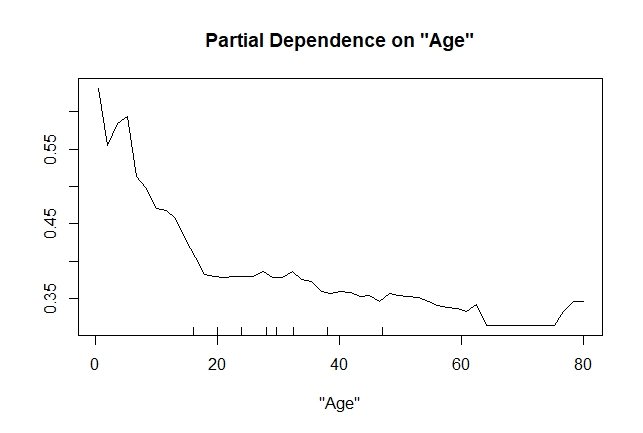
\includegraphics{PDP_Age.jpeg} The PDP shows that young children had the
highest survival probability, with the probability sharply dropping
until age 18. After this age, the decline in survival probability as age
goes up is still evident, but less pronounced.

In classification problems with probability outputs, the partial
dependence function is modeled separately for all of the K different
classes, i.e.~it shows the probability for each respective class at
given feature values of \(x_S\).\footnote{Hastie, Tibshirani, Friedman.
  The Elements of Statistical Learning. Springer.
  \url{https://web.stanford.edu/~hastie/ElemStatLearn/printings/ESLII_print12.pdf}.}
For instance, in the plot below it is clear the passengers in 1st class
had the highest probability of survival and the 3rd class passengers the
lowest.

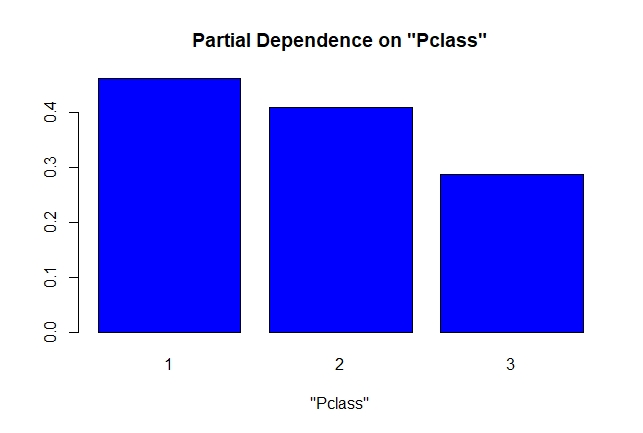
\includegraphics{PDP_Pclass.jpeg} In the categorical PDP, it is clear
that those in lower classes had a lower survival probability.

\textbf{Advantages and Limitations of Partial Dependence Plots}

Partial Dependence Plots are easy to compute and a poular way to explain
insights from black box Machine Learning models. With their intuitive
character, PDPs perfectly qualify for the communication to non-technical
audience. However, due to limited visualization techniques and the
restriction of human perception to a maximum of three dimensions, only
one or two features can reasonably be displayed in one PDP.\footnote{Molnar.
  ``Interpretable Machine Learning''.
  \url{https://christophm.github.io/interpretable-ml-book/simple.html}.}

\begin{figure}
\centering
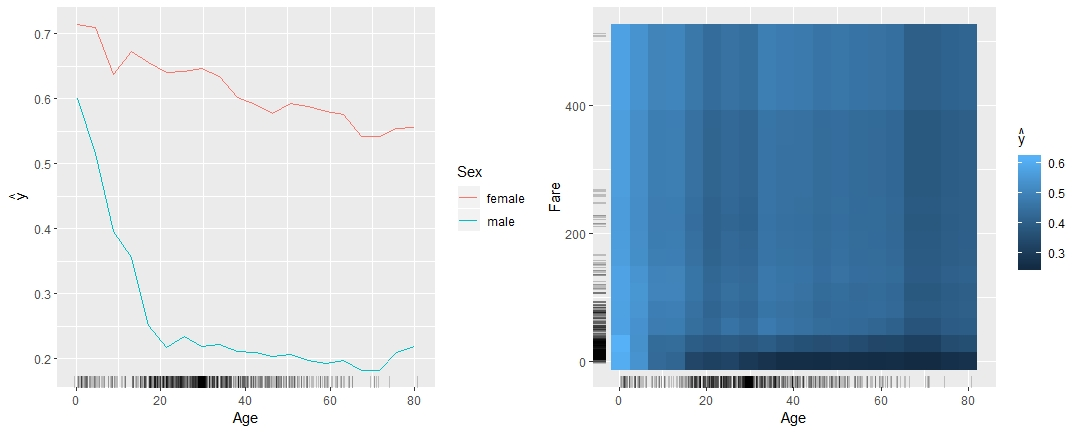
\includegraphics{2_feature_pdp.jpeg}
\caption{2 Feature PDP}
\end{figure}

In the left PDP we see a stark difference in survival probability for
female and male. While for both genders the probability goes down as age
increases, this decrease is much more steep for males. In the right plot
we see that the age range 0-20 has a fairly uniform probability,
independent of the fare paid. From age 20 onwards, however, it is clear
that those that paid the absolute lowest fare had a much lower survival
probability than those that paid a high fare.

Drawing a PDP with one or two feature variables allows a
straight-forward interpretation of the marginal effects. This holds true
as long as the features are not correlated. Should this assumption be
violated, the partial dependence function will produce unrealistic data
points. Furthermore, opposite effects of heterogeneous subgroups might
remain hidden through averaging the marginal effects, which could lead
to wrong conclusions.\footnote{Molnar. ``Interpretable Machine
  Learning''.
  \url{https://christophm.github.io/interpretable-ml-book/simple.html}.}

{[}PLOT: PDP with correlated features{]}

\section{Individual Conditional Expectation
Curves}\label{individual-conditional-expectation-curves}

A formal definition: In ICE plots, for each instance in
\({(x^{(i)}_S, x^{(i)}_C)}^N_{i=1}\), the curve \(\hat{f}_S^{(i)}\) is
plotted against \(x^{(i)}_S\) and \(x^{(i)}_C\).\footnote{Molnar.
  ``Interpretable Machine Learning''.
  \url{https://christophm.github.io/interpretable-ml-book/simple.html}.}

Individual Conditional Expectation (ICE) plots display one line per
instance that shows how the instance's prediction changes when a feature
changes.

The equivalent to a PDP for individual data instances is called
individual conditional expectation (ICE) plot (Goldstein et al.
2017)\footnote{Goldstein, Alex, et al. ``Peeking inside the black box:
  Visualizing statistical learning with plots of individual conditional
  expectation.'' Journal of Computational and Graphical Statistics 24.1
  (2015): 44-65.}. An ICE plot visualizes the dependence of the
prediction on a feature for each instance separately, resulting in one
line per instance, compared to one line overall in partial dependence
plots. A PDP is the average of the lines of an ICE plot. The values for
a line (and one instance) can be computed by keeping all other features
the same, creating variants of this instance by replacing the feature's
value with values from a grid and making predictions with the black box
model for these newly created instances. The result is a set of points
for an instance with the feature value from the grid and the respective
predictions.

\subsection{Centered ICE Plot}\label{centered-ice-plot}

There is a problem with ICE plots: Sometimes it can be hard to tell
whether the ICE curves differ between individuals because they start at
different predictions. A simple solution is to center the curves at a
certain point in the feature and display only the difference in the
prediction to this point. The resulting plot is called centered ICE plot
(c-ICE). Anchoring the curves at the lower end of the feature is a good
choice. The new curves are defined as:
\[\hat{f}^{(i)}_{cent} = \hat{f}^{(i)} - \mathbb{1}\hat{f}(x^a,x^{(i)}_C)\]

\subsection{Derivative ICE Plot}\label{derivative-ice-plot}

\subsection{Advantages and
Disadvantages}\label{advantages-and-disadvantages}

\subsection{ICE}\label{ice}

\begin{figure}
\centering
\includegraphics{ice_plots.jpeg}
\caption{ICE}
\end{figure}

In the 0-50 range in the centered plot we see some variation with some
individual's survival probalility increasing as the fare goes up, while
decreasing for other individuals. After this the curves move more
uniform, with very little changes in the 100-350 range. A small uptick
in surival probality for all individuals takes place at a fare of
roughly 390, before stabilizing for the rest of the range.

\chapter{Accumulated Local Effects
(ALE)}\label{accumulated-local-effects-ale}

\chapter{Permutation Feature Importance and
LOCO}\label{permutation-feature-importance-and-loco}

\section{Permutation Feature
Importance}\label{permutation-feature-importance}

\section{Leave-One-Covariate-Out
(LOCO)}\label{leave-one-covariate-out-loco}

\chapter{Local Interpretable Model-agnostic
Explanations}\label{local-interpretable-model-agnostic-explanations}

\bibliography{book.bib,packages.bib}

\backmatter
\printindex

\end{document}
